% vim: set fenc=utf-8 ft=latex
% !Mode:: "TeX:UTF-8"
% !TEX encoding = UTF-8 Unicode
% -*- mode: latex -*-
% -*- coding: UTF-8 -*-
% kate: encoding utf-8;
%
% IMPORTANT Note: This file is UTF-8 encoded!
%                 You should see some umlauts here: ÄÖÜäöü

\documentclass{beamer}
\usepackage[utf8]{inputenc}

%%%%%%%%%%%%%%%%%%%%%%%%%%%%%%%%%%%%%%%%
% Metadata
%
\title{Feingranularer Zuschnitt von Brot}
\subtitle{Brotscheiben: Considered Harmful}

  \author[dietrich@cs.fau.de]{Christian Dietrich}

  \institute[FAU]{
    System Software Group \\
    Friedrich-Alexander University Erlangen-Nuremberg (FAU)
  }
  \date[Juni '14]{CS 4 - FAU}


%%%%%%%%%%%%%%%%%%%%%%%%%%%%%%%%%%%%%%%%
% Fonts and typesetting
%
  \usepackage[T1]{fontenc}
  \usepackage{lmodern}
  \usepackage{charter}
%  \renewcommand{\sfdefault}{cmbr}
  \usepackage[scaled=0.85]{beramono}
  \usepackage{csquotes}
  \MakeOuterQuote{"}

  \usepackage{slashed}

%%%%%%%%%%%%%%%%%%%%%%%%%%%%%%%%%%%%%%%%
% beamer and beamertools setup
%
  \usecolortheme{rose}
  \usetheme{i4}
  \setbeamertemplate{navigation symbols}{}
  \PassOptionsToPackage{adjustbox}{export}
  \usepackage{beamertools}
  \btset{every block/.append style={shaded transition=false, align=center}}

  \newcommand{\InsertAgenda}[1][\empty]{
    \frame{
      \frametitle{Agenda}
      \tableofcontents[sectionstyle=show/shaded, #1]
    }
  }
  \def\InsertFrameNumber{\insertframenumber}


%%%%%%%%%%%%%%%%%%%%%%%%%%%%%%%%%%%%%%%%
% TikZ setup
%
  \usepackage{tikz}
  % common settings are shared with external TikZ figures
  \input{tikz.styles}

%%%%%%%%%%%%%%%%%%%%%%%%%%%%%%%%%%%%%%%%
% Misc
%
  \usepackage{calc,linegoal}

%%%%%%%%%%%%%%%%%%%%%%%%%%%%%%%%%%%%%%%%
% biblatex setup
%
\usepackage[doi=true,style=alphabetic,isbn=true,abbreviate=false,maxbibnames=99,mincrossrefs=999,sortcites]{biblatex}

    % basic formatting
    \defbibheading{bibliography}{}
    \renewcommand{\bibfont}{\scriptsize}
    \DeclareFieldFormat{postnote}{#1}

    % define \citeautor*, which prints out only the firstauthor, regardless of the maxnames setting
    \DeclareCiteCommand*{\citeauthor}
      {\defcounter{maxnames}{1}%
       \defcounter{minnames}{1}%
       \boolfalse{citetracker}%
       \boolfalse{pagetracker}%
       \usebibmacro{prenote}}
      {\ifciteindex
         {\indexnames{labelname}}
         {}%
       \printnames{labelname}}
      {\multicitedelim}
      {\usebibmacro{postnote}}

    \bibliography{references}

    % tailor content of bib entries
    \AtEveryBibitem{
      \clearfield{month}
      \clearfield{series}
      \clearfield{venue} % <- removed
      \clearfield{eventday}
      \clearfield{isbn}
      \clearfield{eventmonth}
      % \clearfield{eventyear}
      % \clearfield{pages} % <- removed
      \clearname{editor}
      % \clearlist{publisher}
      \clearlist{location} % alias to field 'address'
    }

%
% End of preamble
%%%%%%%%%%%%%%%%%%%%%%%%%%%%%%%%%%%%%%%%

\begin{document}



\begin{frame}[plain]
  \titlepage


\end{frame}

\section{Introduction}

\begin{frame}{Special-Purpose Systems}
  \centering
  \adjustimage{width=\textwidth,max height=\textheight}{fig/blue-gene}
  \RedBox<2>[putat={(1.5cm,5cm)}, text width=0.9\textwidth, fill opacity=0.9, scale content=0.95]{%
    \setlength{\leftmargini}{3ex}
    \bi
      \ii Diversity of applications
      \ii Heterogeneity of hardware platforms
      \ii Some Citation:~\cite{scheler:11:phd}

      \ii[]
      \large
      \ii \textcolor{i4blue}{\bfseries How to reflect this in the design of system software?}
    \ei
  }

\end{frame}


\section[BrOT]{BrOT: An Breakable Operating System Technique}
\def\insertsection{BrOT}
\InsertAgenda

\begin{frame}{Brotly Computing: Korn}
  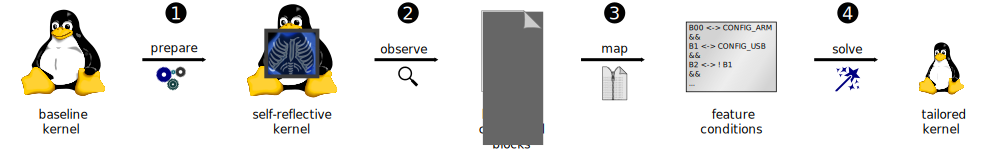
\includegraphics[width=\linewidth]{fig/toolchain.pdf} % Build from SVG
\end{frame}


\section[Conclusion]{Conclusion}
\def\insertsection{Conclusion}
\InsertAgenda

\begin{frame}{Conclusion}
  \includegraphics{fig/minimal}
\end{frame}




%======================================================================

\begin{frame}[allowframebreaks]
  \frametitle {Bibliography}
  \printbibliography
\end{frame}

\end{document}
